\documentclass[9pt]{beamer}
\usetheme[progressbar=frametitle]{metropolis}
\usepackage{appendixnumberbeamer}
\usepackage[small,bf]{caption}
\usepackage{UWMetropolis}

\usepackage{movie15}
% \usepackage{multimedia}

\usepackage[numbers,sort&compress]{natbib}
\usepackage[english]{babel}
\usepackage{pgfplots}	
\usepackage{subfig}
\usepackage{float}
\usepackage{array}
\usepackage{makecell}
\usepackage{mathtools}
\usepackage{tikz}
\usetikzlibrary{tikzmark,shapes,positioning}
\usepackage{multirow}

% \usepackage{movie15}


\newcommand{\flag}{0}% 0 for class, 1 for workshop
\newcommand{\redpause}{\addtocounter{beamerpauses}{-1}\pause\color<+>{red}}

\newcommand{\propnumber}{} % initialize
\newtheorem{prop}{Proposition \propnumber}

\newtheorem{assum}{Assumption}

\setbeamercolor{block title}{use=structure,fg=white,bg=structure.fg!75!uwpurple}
\setbeamercolor{block body}{parent=normal text,use=block title,bg=block title.bg!10!bg}

\addtocounter{figure}{1}

\usepackage{booktabs}
\usepackage[scale=2]{ccicons}

\usepackage{xspace}
\newcommand{\themename}{\textbf{\textsc{metropolis}}\xspace} % Can be removed

\title{Decentralized Multi-Robot Task Assignment (MRTA)}
\subtitle{PhD Qualifying Exam}
\date{\today}
\author{\textbf{Mohamed Safwat}}
\institute{Department of Mechanical Engineering, \\ University of Washington Seattle}
\titlegraphic{
    \hfill
	
\includegraphics[scale=0.35]{UWLogo.eps}
}
\setbeamercovered{transparent}

\input defs.tex

\begin{document}

\maketitle
\setbeamercolor{progress bar}{fg=uwgold,bg=uwmetallicgold}

\begin{frame}{Table of contents}
  \setbeamertemplate{section in toc}[sections numbered]
  \tableofcontents[hideallsubsections]
\end{frame}

\section{Literature Review}
%%%%%%%%%%%%%%%%%%% Background
%%%%%%%%%%%%%%%%%%%

\begin{frame}{Literature Review - Background on MRTA}
    \begin{itemize}
        \item Assign $N_u$ robots to $N_t$ tasks to maximize a global reward with application-specific constraints
        % \item Constraints are domain specific
        \item Some applications of the MRTA,

        \begin{figure}
            \centering
            \subfloat[Package delivery~\cite{DeliveryRobots, bai2019efficient, camisa2022multi}]{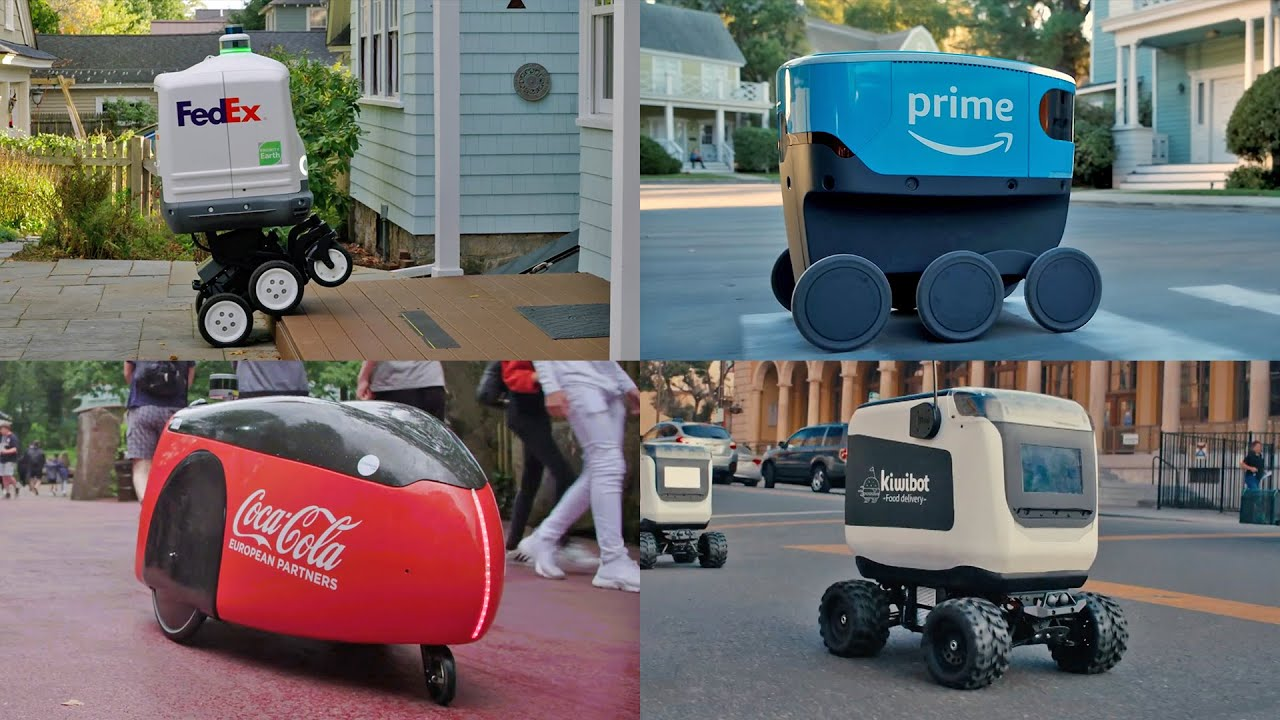
\includegraphics[width=0.37\linewidth]{Figures/delivery_robots.jpg}}
            \hspace{0.3pt}
            \subfloat[Transporting products~\cite{WarehouseRobots, coltin2013online}]{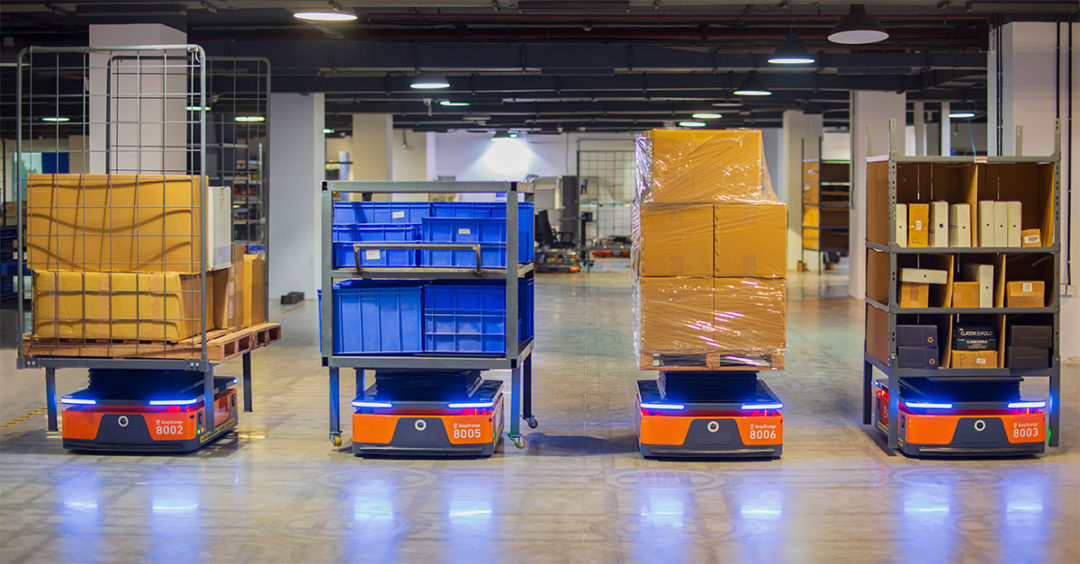
\includegraphics[width=0.4\linewidth]{Figures/warehouse robots.jpg}}
            \vfill
            \subfloat[Wildfire tracking and management~\cite{DronesWildfire,chen2024drone}]{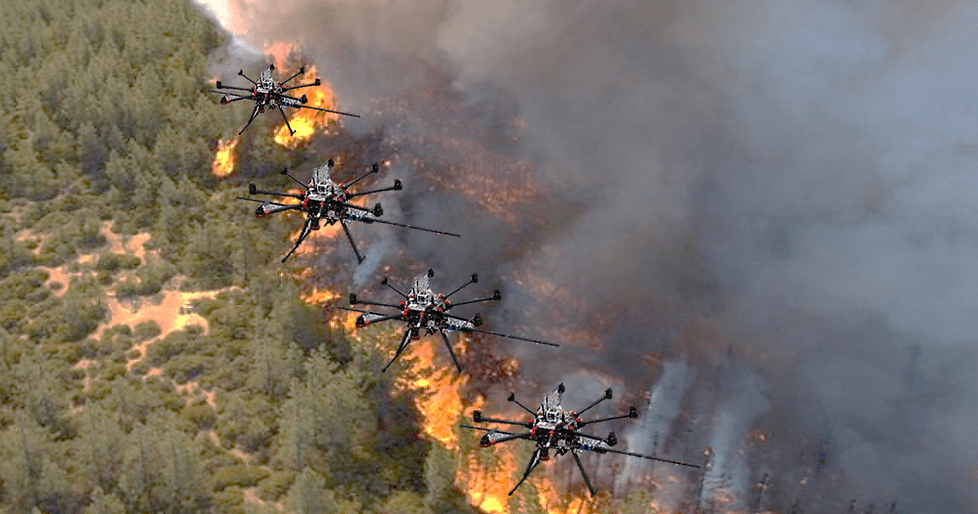
\includegraphics[width=0.37\linewidth]{Figures/Drones-and-wildfire.png}}
            \hspace{0.3pt}
            % \subfloat[Search and rescue operations ~\cite{SearchRescue}]{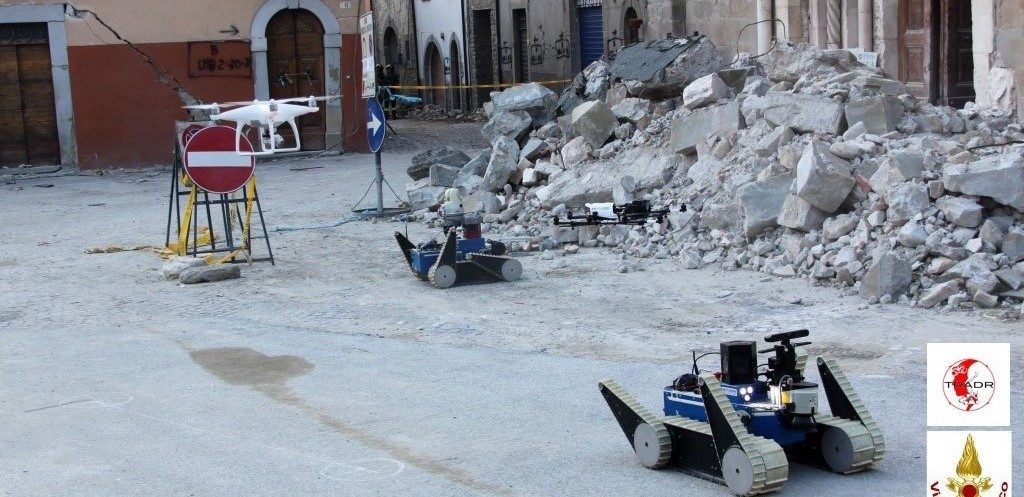
\includegraphics[width=0.4\linewidth]{Figures/search_rescue.jpg}}
        \end{figure}
        % \begin{figure}
        %     \centering
        %     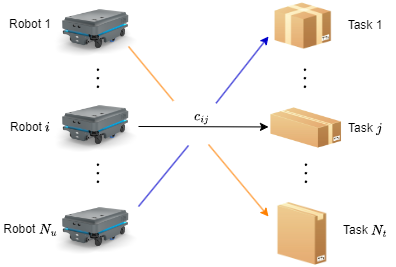
\includegraphics[width=0.5\linewidth]{Figures/Single assignment problem.png}
        % \end{figure}
    \end{itemize}
\end{frame}

%%%%%%%%%%%%%%%%%%% Background
%%%%%%%%%%%%%%%%%%%

\begin{frame}{Literature Review - Formulation}
\begin{itemize}
    \item Combinatorial optimization problem with binary decision variables $x_{ij}$
\end{itemize}
 \vspace{4pt}
    \begin{columns}
    \begin{column}{0.65\textwidth}
    % \begin{itemize}
        % \item Combinatorial optimization problem with binary decision variables $x_{ij}$, \\
        \begin{subequations}
            \label{eq_opt_problem}
            \begin{align}
            \redpause
            & \max \quad \sum_{i=1}^{N_u} \sum_{j=1}^{N_t} \tikzmarknode[uwpurple]{cij}{c_{ij}}(\mathbf{x}_i, \tikzmarknode[uwpurple]{p_i}{\mathbf{p}_i})\cdot x_{ij} \\ \redpause
            & \text{s.t} \quad \sum_{j=1}^{N_t} x_{ij} \leq \tikzmarknode[uwpurple]{L_t}{L_t} \quad \forall i \in %\mathcal{I} \triangleq 
            \{1,\cdots,N_u\}, \\ \redpause
            & \qquad \sum_{i=1}^{N_u} x_{ij} \leq 1 \quad \forall j \in %\mathcal{J} \triangleq 
            \{1,\cdots,N_t\}, \\ \redpause
            & \qquad \sum_{i=1}^{N_u} \sum_{j=1}^{N_t} x_{ij} = 
            %N_{\min} \triangleq 
            \min \{N_t, N_u\cdot L_t\}  \\ \redpause
            & \qquad x_{ij} \in \{0, 1\} \quad \forall (i,j) 
            %  \in \mathcal{I} \times \mathcal{J},
            \end{align}
        \end{subequations}
        \begin{tikzpicture}[overlay, remember picture]
            \onslide<1->
            \node[above right=0.36cm and -2.5cm of cij, align=center, color=uwpurple] (label) {\footnotesize score function: reward for robot $i$ completing task $j$};
            \draw[->, thick, uwpurple] (label) -- (cij);
            \node[below right=0.36cm and -1.8cm of p_i, align=center, color=uwpurple] (label2) {\footnotesize path vector (order of task execution) };
            \draw[->, thick, uwpurple] (label2) -- (p_i);
            \onslide<2->
            \node[below right=0.36cm and -1.0cm of L_t, align=center, color=uwpurple] (label3) {\footnotesize max. \# of tasks each robot can get};
            \draw[->, thick, uwpurple] (label3) -- (L_t);
        \end{tikzpicture}
        \onslide<5->
        % \item Can be more general (e.g., robot coalitions)
    % \end{itemize}
    \end{column}
    \begin{column}{0.55\textwidth}
        % \begin{figure}
        %     {
        %     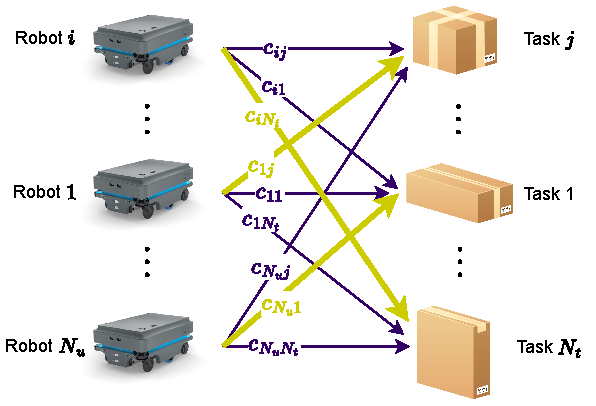
\includegraphics[width=0.62\linewidth]{Figures/LinearAssign.pdf}}
        %     \caption{Linear single assignment ($L_t=1$) with constant score values}
        % \end{figure}
        \begin{figure}
            \centering
            \onslide<1->
            \subfloat[Linear single assignment ($L_t=1$) with constant score values ]{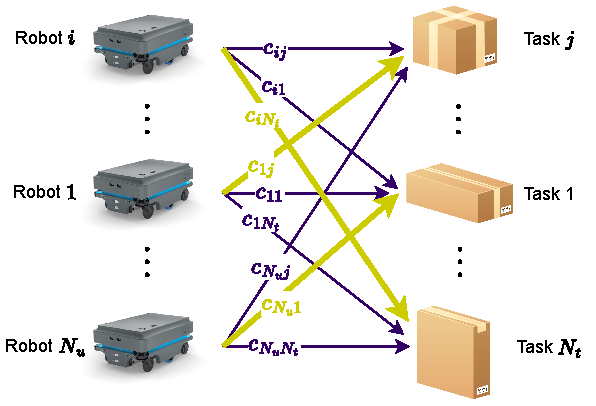
\includegraphics[width=0.85\linewidth]{Figures/LinearAssign.pdf}}
            \addtocounter{subfigure}{-1}
            \vfill
        % \label{fig:1}
        \end{figure}
    \end{column}
    \end{columns}
\end{frame}

%%%%%%%%%%%%%%%%%%% Applications
%%%%%%%%%%%%%%%%%%%
\begin{frame}{Literature Review - Centralized MRTA}
    \begin{columns}
    \begin{column}{0.65\textwidth}
    \begin{itemize}
        % \item Centralized task assignment (TA)
        \item Task assignment (TA) is NP-Hard~\cite{karp2010reducibility} (even the linear TA)
        \item Linear assignment $c_{ij}(\mathbf{x}_i,{\mathbf{p}_i}) = c_{ij}$ 
        \begin{itemize}
            \item Can be solved efficiently in some cases~\cite{bertsekas1991linear}
            \item Linear program relaxation: $x_{ij} \in \{0, 1\}$ to $0\le x_{ij} \le 1$
            \item Hungarian method~\cite{kuhn1955hungarian}, auction algorithm~\cite{bertsekas1988auction}
        \end{itemize}
        \vspace{0.4cm}
        \pause
        \item Nonlinear assignment
        \begin{itemize}
            \item Exact methods: dynamic programming~\cite{pardalos1999nonlinear}, branch and bound ~\cite{dyer1986linear} (exponential complexity)
            \item Approximate methods: convex relaxations~\cite{ma2015efficient}, greedy algorithms~\cite{romeijn2000class}
            % \item For example, $c_{ij}(\mathbf{x}_i,{\mathbf{p}_i})$ can be the probability that a set of robots successfully complete a task~\cite{haight2000integer} 
        \end{itemize}
    \end{itemize}
    \end{column}
    \begin{column}{0.5\textwidth}
    \begin{figure}
        \centering
        \onslide<1->
        \subfloat[Linear MRTA (one to one)]{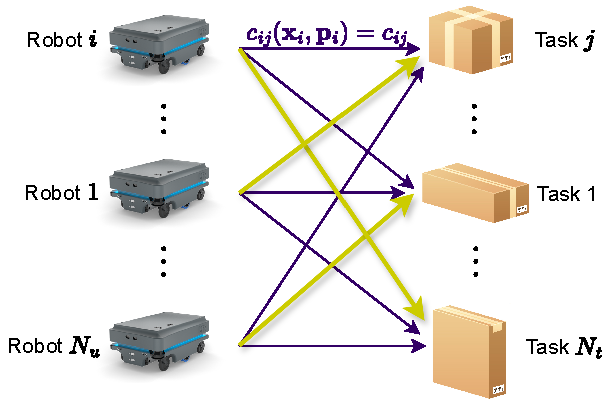
\includegraphics[width=0.8\linewidth]{Figures/LinearAssign_2.pdf}}
        \vfill
        \visible<2>{
        \subfloat[Nonlinear MRTA (robot coalitions)]{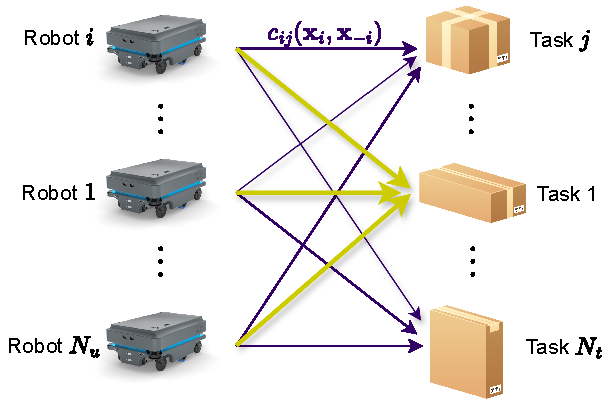
\includegraphics[width=0.8\linewidth]{Figures/nonlinearAssign.pdf}}
        }
    % \label{fig:1}
    \addtocounter{subfigure}{-1}
    \end{figure}
    \end{column}
    \end{columns}
\end{frame}

\begin{frame}{Literature Review - Decentralized MRTA}
    \begin{itemize}
        \item Decentralized MRTA methods are becoming more relevant
        \begin{itemize}
            \item Computationally efficient~\cite{choi2009consensus}; robust~\cite{chopra2017distributed}; scalable~\cite{shorinwa2023distributed}
        \end{itemize}
        % \item Derived from their centralized counterpart
        % \item Implicit methods: coordination on local information
        % \item Explicit methods: coordination on local understanding of assignments
    \end{itemize}

    \begin{block}{~\vspace{0.2cm}}
        \begin{center}
        \vspace{-1.0cm}
        \setcellgapes{3pt}\makegapedcells
        \begin{tabular}{>{\centering}p{0.45\textwidth}|>{\centering\arraybackslash}p{0.45\textwidth}}
         \textcolor{white}{\bfseries\boldmath Implicit methods~\cite{alighanbari2005decentralized, curtis2003simultaneous, samiei2023distributed}} & \textcolor{white}{\bfseries Explicit methods~\cite{arslan2007autonomous,choi2009consensus,johnson2017decentralized, shorinwa2023distributed, qu2019distributed}} \\
        consensus on information 
        (e.g., task positions) 
        % to compute score function matrix $C(\mathbf{p},\mathbf{x})\in \reals^{N_u \times N_t}$ 
        & consensus on local understanding of assignments \\ 
        solve local copy of the entire MRTA to get $\mathbf{x}\in \{0,1\}^{N_u \times N_t}$&  each robot solves only for its local assignments $\mathbf{x}_i \in \{0,1\}^{N_t}$
        % either solve a local copy of the entire MRTA to get $\mathbf{x}$ or each robot's local assignments $\mathbf{x}_i \in \{0,1\}^{N_t}$
        \\ \hline
        \begin{itemize}
            \item {\color{ao} high global reward}
            \item {\color{red}conflicting assignments if inaccurate information}
            \item {\color{red}computationally inefficient} 
        \end{itemize}
        &
        \begin{itemize}
            \item {\color{ao}computationally efficient}
            \item {\color{ao}conflict-free assignments}
            \item {\color{red} low global reward because assignments are based on local information}
        \end{itemize}
        
        \end{tabular}
        \end{center}
    \end{block}
\end{frame}

% \begin{frame}{Literature Review - Implicit methods}
%     \begin{columns}
%     \begin{column}{0.6\textwidth}
%     \begin{itemize}
%         \item Distributed Hungarian algorithm~\cite{samiei2023distributed} (similarly~\cite{alighanbari2005decentralized})
%         \begin{itemize}
%             \item Step 1: communicate local information to converge on global information
%             \item Step 2: build score/cost matrix and solve the Hungarian algorithm 
%         \end{itemize}
%         \item {\color{green}Achieves assignments with high global reward}
%         \item {\color{red}Conflicting assignments if inaccurate information communication}
%         \item {\color{red}Computationally inefficient}
%     \end{itemize}
%     \end{column}
%     \begin{column}{0.55\textwidth}
%     \begin{figure}
%         \centering
%         \onslide<1->
%         \subfloat[Communication]{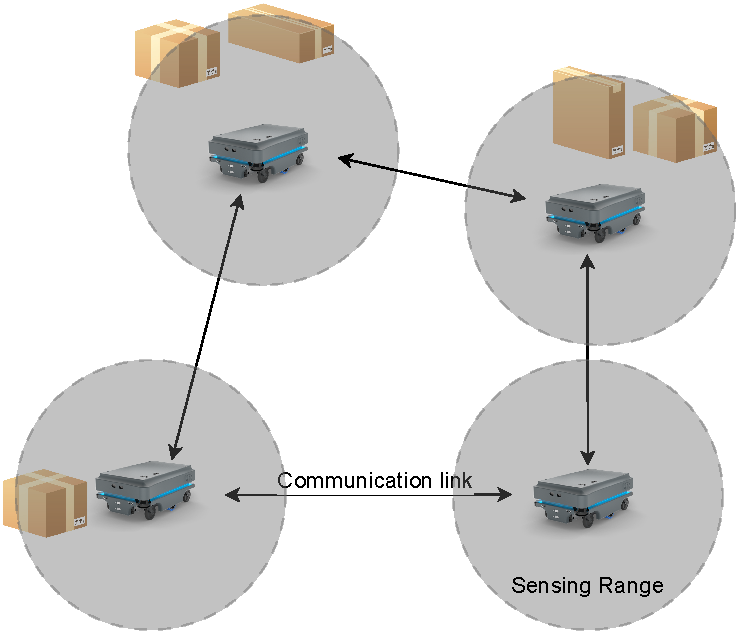
\includegraphics[width=0.7\linewidth]{Figures/communication.pdf}}
%         \vfill
%         \subfloat[Solve locally]{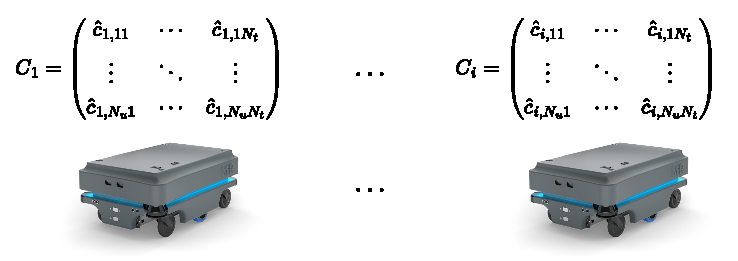
\includegraphics[width=1.\linewidth]{Figures/score_matrices.pdf}}
%     \label{fig:2}
%     \end{figure}
%     \end{column}
%     \end{columns}
% \end{frame}

% \begin{frame}{Literature Review - Explicit methods}
%     \begin{columns}
%     \begin{column}{0.6\textwidth}
%     \begin{itemize}
%         \item Distributed auction algorithms~\cite{choi2009consensus},Game-theoretic~\cite{arslan2007autonomous}, and distributed optimization methods~\cite{shorinwa2023distributed, camisa2022multi}
%         \item High-level idea:
%         \begin{itemize}
%             \item Step 1: each robot locally chooses an assignment 
%             \item Step 2: communicate assignments to resolve conflicts 
%         \end{itemize}
%         \item {\color{green}Computationally efficient}
%         \item {\color{green}Conflict-free assignments}
%         \item {\color{red}Base their assignments on their local information or assume information is globally known}
%     \end{itemize}
%     \end{column}
%     \begin{column}{0.55\textwidth}
%     \begin{figure}
%         \centering
%         \onslide<1->
%         \subfloat[Communication]{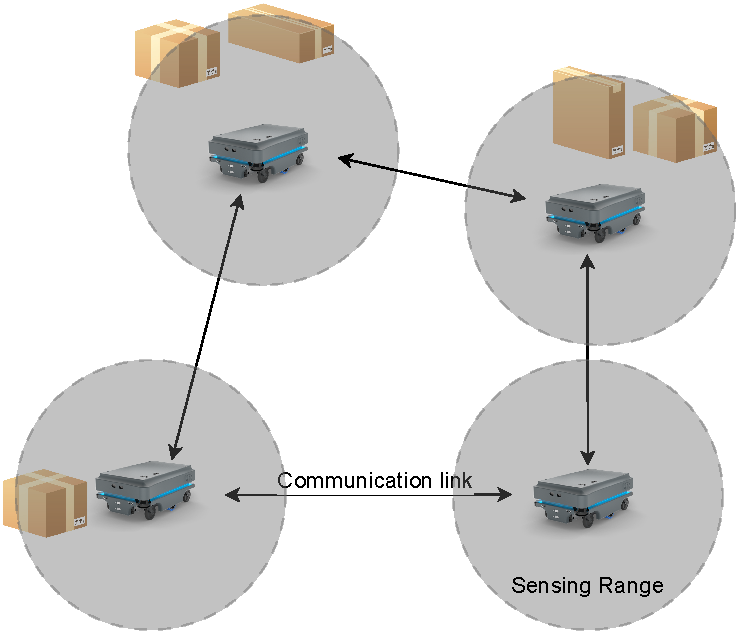
\includegraphics[width=0.7\linewidth]{Figures/communication.pdf}}
%         \vfill
%     \label{fig:2}
%     \end{figure}
%     \end{column}
%     \end{columns}
% \end{frame}

\section{Paper Review}
\begin{frame}{Paper Review}
    ``Consensus-Based Decentralized Auctions for Robust Task Allocation" by  Choi et al. \cite{choi2009consensus}
    \begin{itemize}
        \item Assignment Algorithm
        \item Guarantees
        \item Numerical Results
        \item Strengths and Weaknesses 
    \end{itemize}
\end{frame}

% \begin{frame}{Paper Review - CBAA}
%     \begin{columns}
%     \begin{column}{0.65\textwidth}
%     \begin{itemize}
%         \item CBAA is for the single linear assignment problem in Eq.~\eqref{linear_assign} consisting of auction and consensus phases
%         \pause
%         \item Auction phase: 
%         \begin{itemize}
%             \item Each robot has a local winning bid list $\mathbf{y}_i \in \reals_{+}^{N_t}$
%             \item Independently choose an unassigned task with the largest $c_{ij} \in \reals_{+}$ and $c_{ij} > y_{ij}$ (denote this task $J_i$)
%             \item Update component $y_{i,J_i} = c_{i,J_i}$
%         \end{itemize} 
%         \pause
%         \item Consensus phase: 
%         \begin{itemize}
%             \item Communicate winning bid list $\mathbf{y}_i$ with neighbors 
%             \item Do maximum consensus on the components of $\mathbf{y}_i$
%             \item Loose task assignment if another robot has a higher bid
%         \end{itemize} 
%     \end{itemize}
%     \end{column}
%     \begin{column}{0.5\textwidth}
%     \onslide<1->
%     \begin{equation}
%             \label{linear_assign}
%             \begin{aligned}
%             & \max \quad \sum_{i=1}^{N_u} \sum_{j=1}^{N_t} {\color{red}c_{ij}} \cdot x_{ij} \\
%             % &  \\
%             & \text{s.t} \quad \sum_{j=1}^{N_t} x_{ij} \leq {\color{red}L_t = 1} \quad \forall i \in \mathcal{I}, \\
%             & \sum_{i=1}^{N_u} x_{ij} \leq 1 \quad \forall j \in \mathcal{J}, \\
%             & \sum_{i=1}^{N_u} \sum_{j=1}^{N_t} x_{ij} = \min \{N_t, N_u\},  \\ 
%             & x_{ij} \in \{0, 1\} \quad \forall (i,j) \in \mathcal{I} \times \mathcal{J}.
%             \end{aligned}
%     \end{equation}
%     \end{column}
%     \end{columns}
% \end{frame}

\begin{frame}{Paper Review - CBBA}
    \begin{itemize}
        \item Introduces Consensus-Based Auction Algorithm (CBAA) for the linear single-assignment 
       \begin{figure}
            \centering
            {
            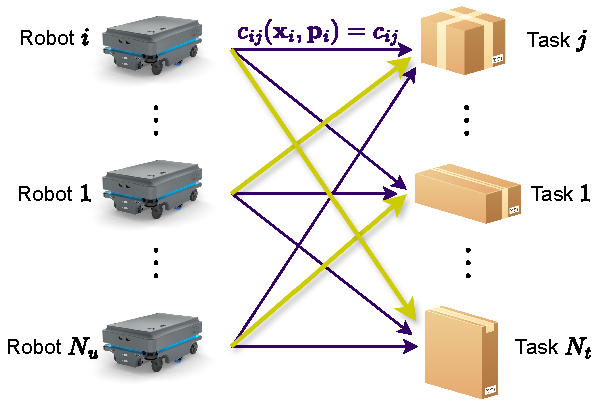
\includegraphics[width=0.4\linewidth]{Figures/CBAA.pdf}}
            % \caption{CBAA for single assignment (left), CBBA for multi assignment (right) }
        \end{figure}
        \pause
        \item Generalize to Consensus-Based Bundle Algorithm (CBBA) to assign a sequence of tasks in a path vector
        % \begin{itemize}
        %     \item Assignments are done on the task level, not the bundle level
        % \end{itemize}
        \visible<2>{
        \begin{figure}
            \centering
            {
            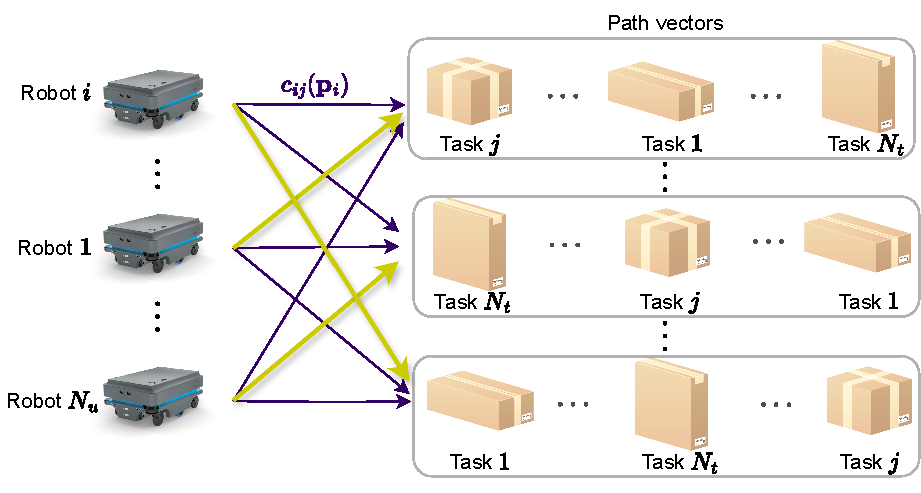
\includegraphics[width=0.62\linewidth]{Figures/CBBA.pdf}}
            % \caption{CBAA for single assignment (left), CBBA for multi assignment (right) }
        \end{figure}}
        
        % \item Scoring function depends on the path vector, i.e., $c_{ij}(\mathbf{p}_i)$ 
        % \item CBBA does the TA on the task level, not the vector level
        % \item Each robot has,
        % \begin{itemize}
        %     \item Bundle $\mathbf{b}_i \in (\mathcal{J} \cup \{\emptyset\})^{L_t}$: a list of tasks ordered based on which task was added first
        %     \item Path vector $\mathbf{p}_i \in (\mathcal{J} \cup \{\emptyset\})^{L_t}$: a list of tasks ordered based on their location in the assignment
        % \end{itemize}
    \end{itemize}
\end{frame}

\begin{frame}{Paper Review - CBBA}
    \begin{itemize}
        \item CBBA consists of bundle construction and consensus iterations
        \item Bundle construction (at each iteration):
        \begin{itemize}
            \item Bundle $\mathbf{b}_i$: a list of tasks ordered based on which task was \textbf{added first}
            \item Path vector $\mathbf{p}_i$: a list of tasks ordered based on their \textbf{location in the assignment}
        \end{itemize}
        \visible<2>{
          \begin{figure}
            \centering
            {
            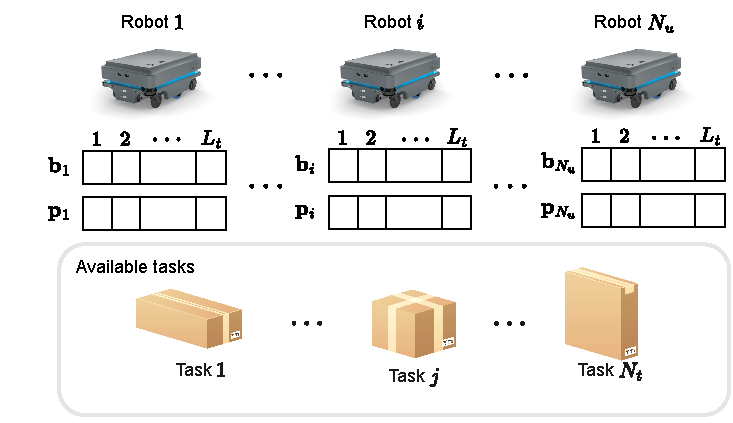
\includegraphics[width=0.9\linewidth]{Figures/bundle_construction_1.pdf}}
        \end{figure}
        }
    \end{itemize}
\end{frame}

\begin{frame}{Paper Review - CBBA}
    \begin{itemize}
        \item CBBA consists of bundle construction and consensus iterations
        \item Bundle construction (at each iteration):
        \begin{itemize}
            \item Bundle $\mathbf{b}_i$: a list of tasks ordered based on which task was \textbf{added first}
            \item Path vector $\mathbf{p}_i$: a list of tasks ordered based on their \textbf{location in the assignment}
        \end{itemize}
          \begin{figure}
            \centering
            {
            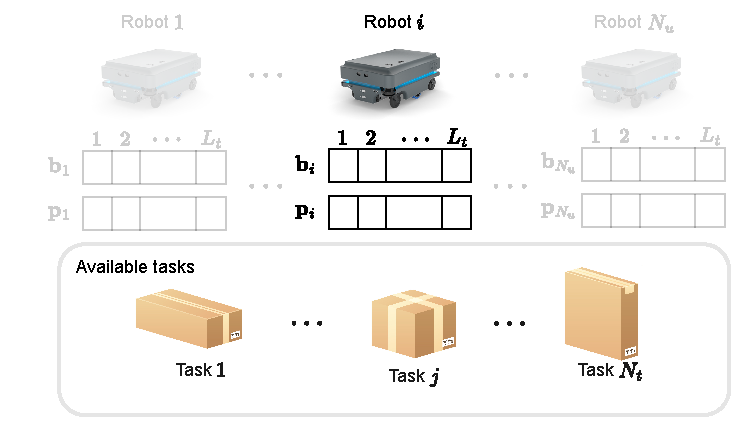
\includegraphics[width=0.9\linewidth]{Figures/bundle_construction_2.pdf}}
        \end{figure}
    \end{itemize}
\end{frame}

\begin{frame}{Paper Review - CBBA}
    \begin{itemize}
        \item Robot $i$ adds unassigned tasks to its bundle and path vector greedily, with the largest marginal score improvement
        \begin{equation*}
            c_{ik}[\mathbf{b}_i] = \max_{n:n\le |\mathbf{p}_i|}\left( \underbrace{S_{i}^{\mathbf{p}_i \oplus_n \{k\}}}_{\text{reward from path $\mathbf{p}_i \oplus_n \{k\}$}} - \underbrace{S_{i}^{\mathbf{p}_i}}_{\text{reward from path $\mathbf{p}_i$}} \right),
        \end{equation*}
        where the best task among all tasks is 
            $k^* = \argmax_{k} \left(c_{ik}[\mathbf{b}_i]\right)$.
        \visible<2>{
        \begin{figure}
            \centering
            {
            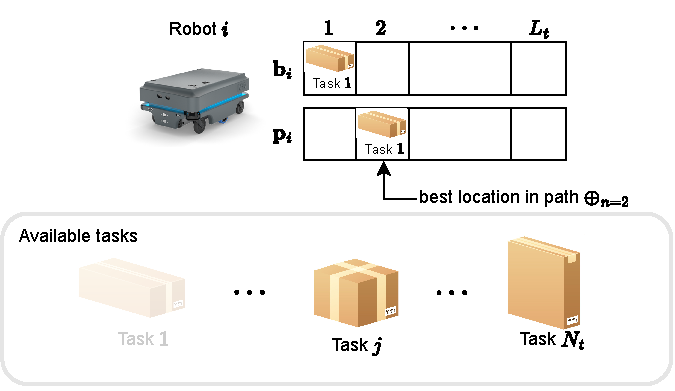
\includegraphics[width=0.85\linewidth]{Figures/bundle_construction_3.pdf}}
        \end{figure}
        }
    \end{itemize}
\end{frame}

\begin{frame}{Paper Review - CBBA}
    \begin{itemize}
        \item Keep adding tasks to the bundle and path vector until they are filled
        \item Robot $i$ also associates each chosen task with itself (for consensus)
        \begin{itemize}
            \item $\mathbf{y}_i$: winning bid list
            \item $\mathbf{z}_i$: winning robot list
        \end{itemize}
        \begin{figure}
            \centering
            {
            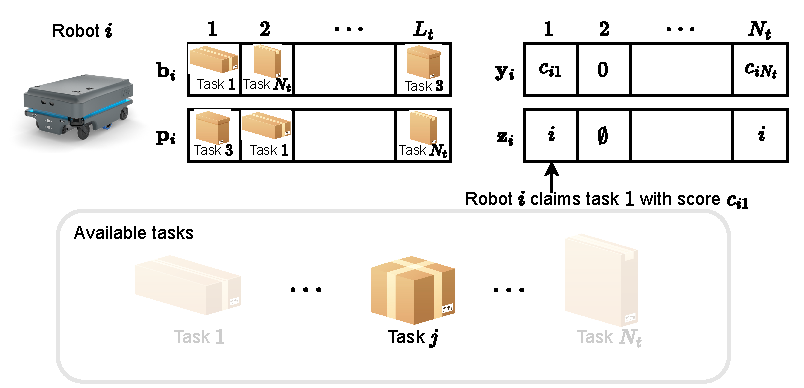
\includegraphics[width=0.95\linewidth]{Figures/bundle_construction_4.pdf}}
        \end{figure}
    \end{itemize}
\end{frame}

\begin{frame}{Paper Review - CBBA}
    \begin{itemize}
        \item Consensus phase for resolving any conflicting task assignments
        \begin{itemize}
            \item Robots communicate
            \begin{itemize}
                \item $\mathbf{y}_i$: winning bid list
                \item $\mathbf{z}_i$: winning robot list
                \item $\mathbf{s}_i$:  time stamp vector for the last information update from other robots
            \end{itemize}
            \pause
            \item Each robot either updates, resets, or keeps its assignment based on $\mathbf{y}_i, \mathbf{z}_i, \mathbf{s}_i$ and decision rules, which are roughly maximum consensus 
        \end{itemize}
        \visible<2>{
        \begin{figure}
            \centering
            {
            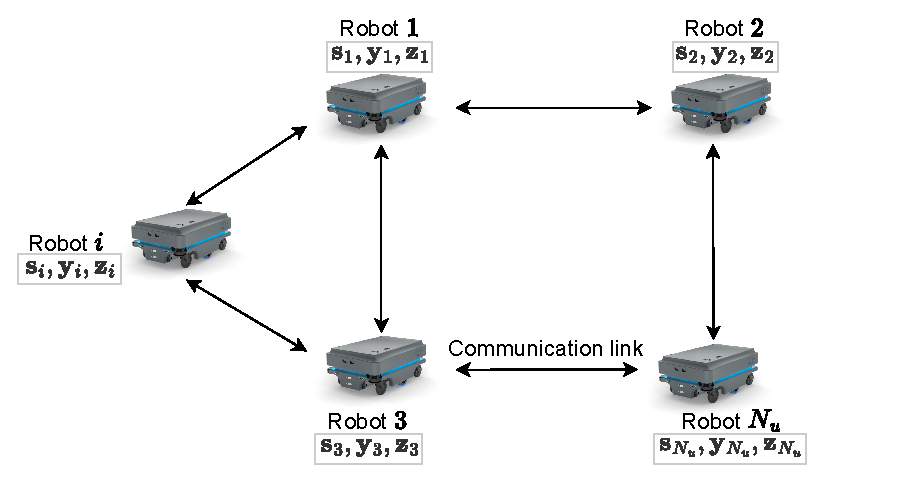
\includegraphics[width=0.95\linewidth]{Figures/consensus_network.pdf}}
        \end{figure}
        }
    \end{itemize}

\end{frame}

\begin{frame}{Paper Review - CBBA Guarantees}
    \begin{itemize}
        \item Two main theorems, convergence and optimally of CBBA, under the following assumption
    \end{itemize}
    \begin{assum}[Diminishing Marginal Gain (DMG) on Scoring Function]
        The value of a task doesn't increase as other elements are added to the set before it, i.e., $$\underbrace{c_{ij}[\mathbf{b}_i]}_{\tiny \text{marginal improvement to } \mathbf{b}_i} \ge \underbrace{c_{ij}[\mathbf{b}_i \oplus_{\text{end}} \mathbf{b}]}_{\tiny \text{marginal improvement to } \mathbf{b}_i \oplus_{\text{end}} \mathbf{b}}$$
    \end{assum}
    \begin{itemize}
        \item The proof of the 2 theorems relies on a reduction of CBBA to a centralized sequential greedy algorithm (SGA).
    \end{itemize}
\end{frame}

\begin{frame}{Paper Review - CBBA Guarantees}
    \begin{theorem}[Convergence of CBBA]
        Provided DMG scoring functions and synchronized consensus over a static communication network
        \begin{columns}
        \begin{column}{0.56\textwidth}
        \begin{enumerate}
            \item CBBA produces the same solution as the sequential greedy algorithm (SGA)
            \item Convergence time is bounded above by $N_{\text{min}} \cdot D = \min \{N_t, N_u\cdot L_t\} \cdot D$ with network diameter $D$
        \end{enumerate}
        \end{column}
        \begin{column}{0.35\textwidth}
        \begin{figure}
            \begin{tikzpicture}[scale=0.65, transform shape]
            % Define the nodes
            \node[draw, circle] (i) at (1,0) {$i$};
            \node[draw, circle] (a) at (2,1) {};
            \node[draw, circle] (b) at (2,-1) {};
            \node[draw, circle] (c) at (4,1) {};
            \node[draw, circle] (d) at (4,-1) {};
            % \node[draw, circle] (e) at (3,1) {}; % New node
            \node[draw, circle] (j) at (5,0) {$m$};
        
            % Draw the edges
            \draw[<->] (i) -- (a);
            \draw[<->] (i) -- (b);
            % \draw (a) -- (c);
            \draw[<->] (b) -- (d);
            \draw[<->] (c) -- (j);
            \draw[<->] (d) -- (j);
            % \draw[<->] (a) -- (e);
            % \draw[<->] (c) -- (e);
            \draw[<->] (a) -- (c);
            % \draw[<->] (c) -- (e);
        
            % Highlight the diameter path
            \draw[line width=2mm, gray, opacity=0.5] (i) -- (b) -- (d) -- (j);
        
            % Add labels
            \node at (3,-0.7) {$D$};
            \end{tikzpicture}
            \caption{Diameter $D$}
        \end{figure}
        \end{column}
    \end{columns}
    \end{theorem}
    \begin{theorem}[Optimality of CBBA]
        Provided DMG scoring functions and accurate situational awareness, CBBA guarantees 50\% optimality for the MRTA.
    \end{theorem}
\end{frame}

\begin{frame}{Paper Review - Numerical Results}
    \begin{itemize}
        \item CBBA is analyzed under inconsistent situational awareness (SA), i.e., position estimates of the tasks among the robots
        \begin{itemize}
            \item Each robot has different estimates of the task positions
        \end{itemize}
    \end{itemize}
    \begin{figure}
        \centering
        \onslide<1->
        \subfloat[Convergence with inconsistent SA]{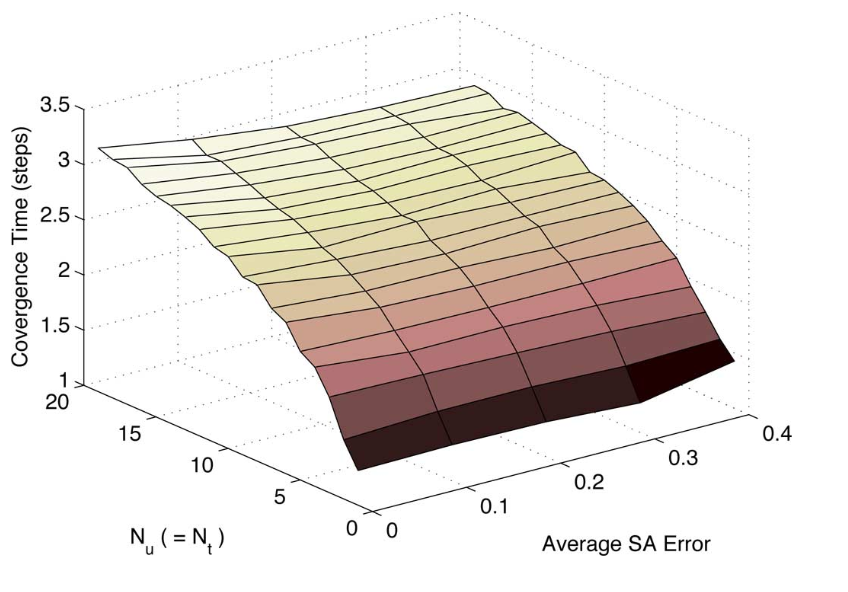
\includegraphics[width=0.45\linewidth]{Figures/convergence_time.png}}
        \hfill
        \subfloat[Optimality gap with inconsistent SA]{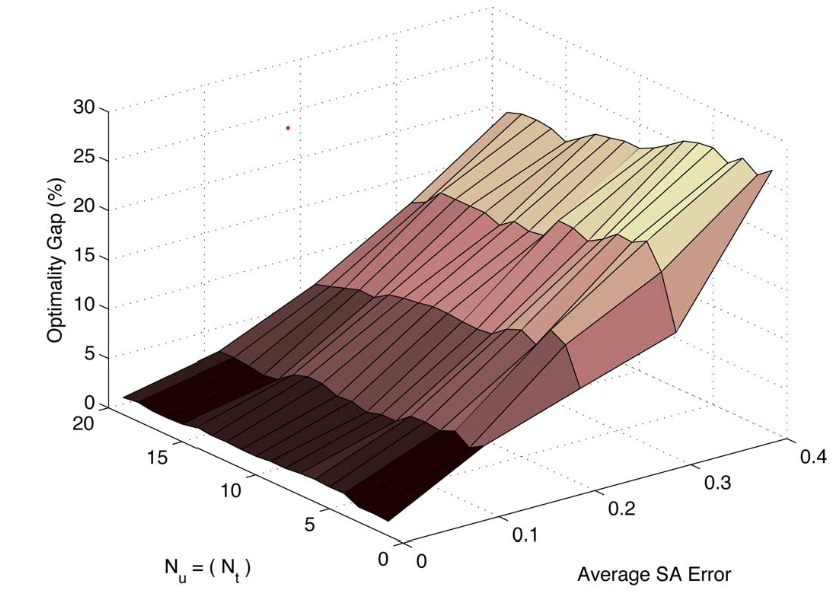
\includegraphics[width=0.45\linewidth]{Figures/optimality_gap.png}}
    \label{fig:2}
    \end{figure}
\end{frame}

\begin{frame}{Paper Review - Strengths and Weaknesses}
    \begin{block}{~\vspace{0.7cm}}
        \begin{center}
        \vspace{-1.0cm}
        \setcellgapes{4pt}\makegapedcells
        \begin{tabular}{>{\centering}p{0.45\textwidth}|>{\centering\arraybackslash}p{0.45\textwidth}}
         \textcolor{white}{\bfseries\boldmath Strengths} & \textcolor{white}{\bfseries Weaknesses} \\
        Computationally efficient %(no need for local copies of the problem)
        &  Assumes local information, i.e., SA relating to score functions, can be sensed/estimated by every robot \\ 
       Guaranteed conflict-free task assignments (even with inconsistent SA) & Score functions need to satisfy the diminishing marginal return property \\  
       Guaranteed to be at least 50\% optimal (although requires consistent SA)
        & 50\% optimal for CBAA (linear assignment case) \\ &  Requires synchronized consensus \\
        & No experiments
        \end{tabular}
        \end{center}
    \end{block}
\end{frame}


\section{Research Plan}
\begin{frame}{Research Plan}
    \begin{itemize}
        \item Explicit (e.g., CBBA) and implicit methods for decentralized MRTA face challenges with dynamic environments
        \begin{itemize}
            \item Explicit methods only allow robots to use local information 
            % \item Standard consensus approaches in implicit methods lead to large errors 
            \pause
            \item Standard consensus in implicit methods lead to zero steady-state error but leads to large errors when the information is changing
        \end{itemize}     
        \begin{equation*}
            \label{standard method}
            \hat{z}_{i,d}[k+1] =  \hat{z}_{i,d}[k] + \gamma \mu_{i,d}[k],   \quad \text{with} \quad \mu_{i,d}[k] = \sum_{j \in \mathcal{N}_i} w_{i,j}\left(\hat{z}_{j,d}[k] - \hat{z}_{i,d}[k]\right).
        \end{equation*}
        \vspace{-0.6cm}
        \visible<2>{
        \begin{figure}[H] 
            \centering
                \subfloat[\label{Fig_standard_1}Standard consensus]{%
               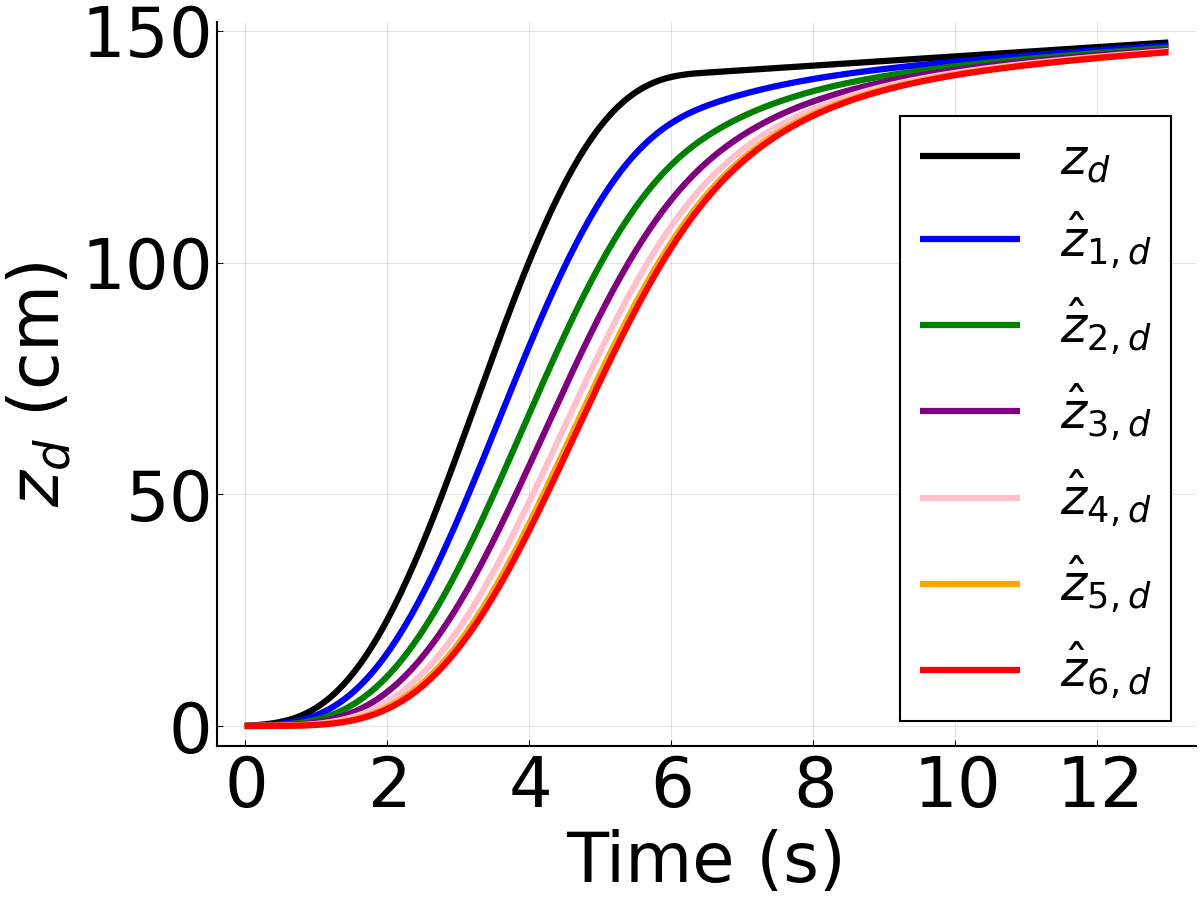
\includegraphics[width=0.4\linewidth]{Figures/standard_quals.png}}

           \subfloat[\label{Communication_network_1}Communication network]{
            \begin{tikzpicture}[>=stealth, scale=0.6, transform shape] % Stealth arrow tips
              % First node (special)
              \node[draw, circle, fill=orange] (zd) at (0,0) {$z_d$};
              
              % Other nodes
              \foreach \x in {1,...,6}
                \node[draw, circle, fill=green, text=black] (\x) at (\x*1.5,0) {$\hat{z}_{\x,d}$};
              
              % Directed edge from zd to 1
              \draw[->] (zd) -- (1);
              
              % Undirected edges from 1 to 6
              \foreach \x [remember=\x as \lastx (initially 1)] in {2,...,6}
                \draw[<->] (\lastx) -- (\x);

            \draw (1) -- node[above] {$w_{1,2}$} (2);
            \end{tikzpicture}

            }
        \end{figure}}
    \end{itemize}
\end{frame}

% \begin{frame}{Research Plan}
%     \begin{itemize}
%         \item Dynamic MRTA in time-varying environments
%         \item Environment is changing and uncertain (e.g., wildfire tracking/management and search and rescue operations) 
%         \begin{itemize}
%             \item Unknown dynamics
%             \item Partial observability
%         \end{itemize}
%          % \item Wildfire tracking and management application: drones collect atmospheric measurements on the canopy of the wildfire and provide a real-time fire spread prediction model~\cite{DronesWildfire}.
%     \end{itemize}
   
%     \begin{figure}
%         \centering
%         \subfloat[~\cite{DronesWildfire,chen2024drone}]
%         {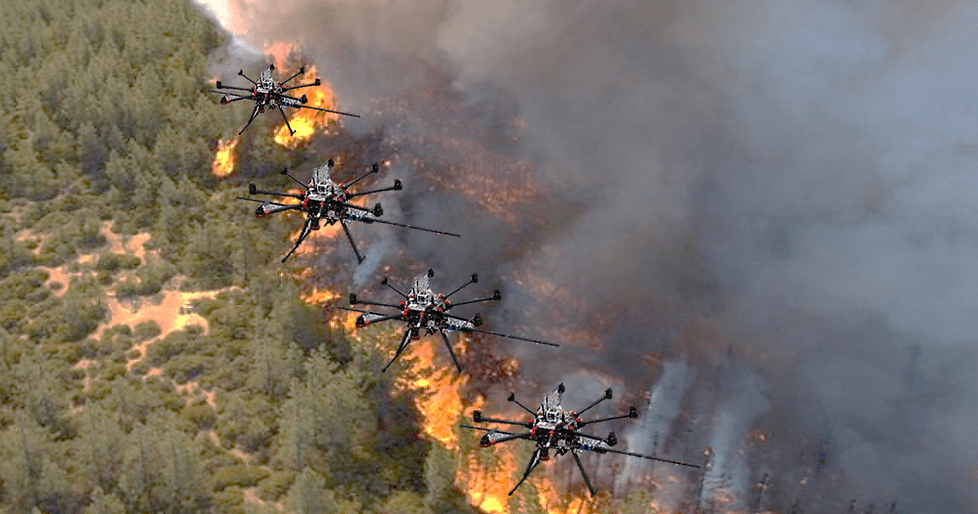
\includegraphics[width=0.5\linewidth]{Figures/Drones-and-wildfire.png}}
%     \end{figure}
% \end{frame}

\begin{frame}{Research Plan}
    \begin{itemize}
        \item Improve the accuracy of the information communicated using delayed-self reinforcement (DSR)~\cite{devasia2020cohesive}
    \end{itemize}
    \begin{equation*}
        \label{dsr method}
        \hat{z}_{i,d}[k+1] =  \underbrace{\hat{z}_{i,d}[k] + \gamma \mu_{i,d}[k]}_{\text{standard method}} + \underbrace{\beta_1 \left(\mu_{i,d}[k] - \mu_{i,d}[k-1]\right) + \beta_2 \left(\hat{z}_{i,d}[k] - \hat{z}_{i,d}[k-1]\right)}_{\text{DSR terms}}.
    \end{equation*}
    \vspace{-0.6cm}
    \begin{figure}[H] 
    \centering
    \subfloat[\label{Fig_standard}Standard consensus]{%
       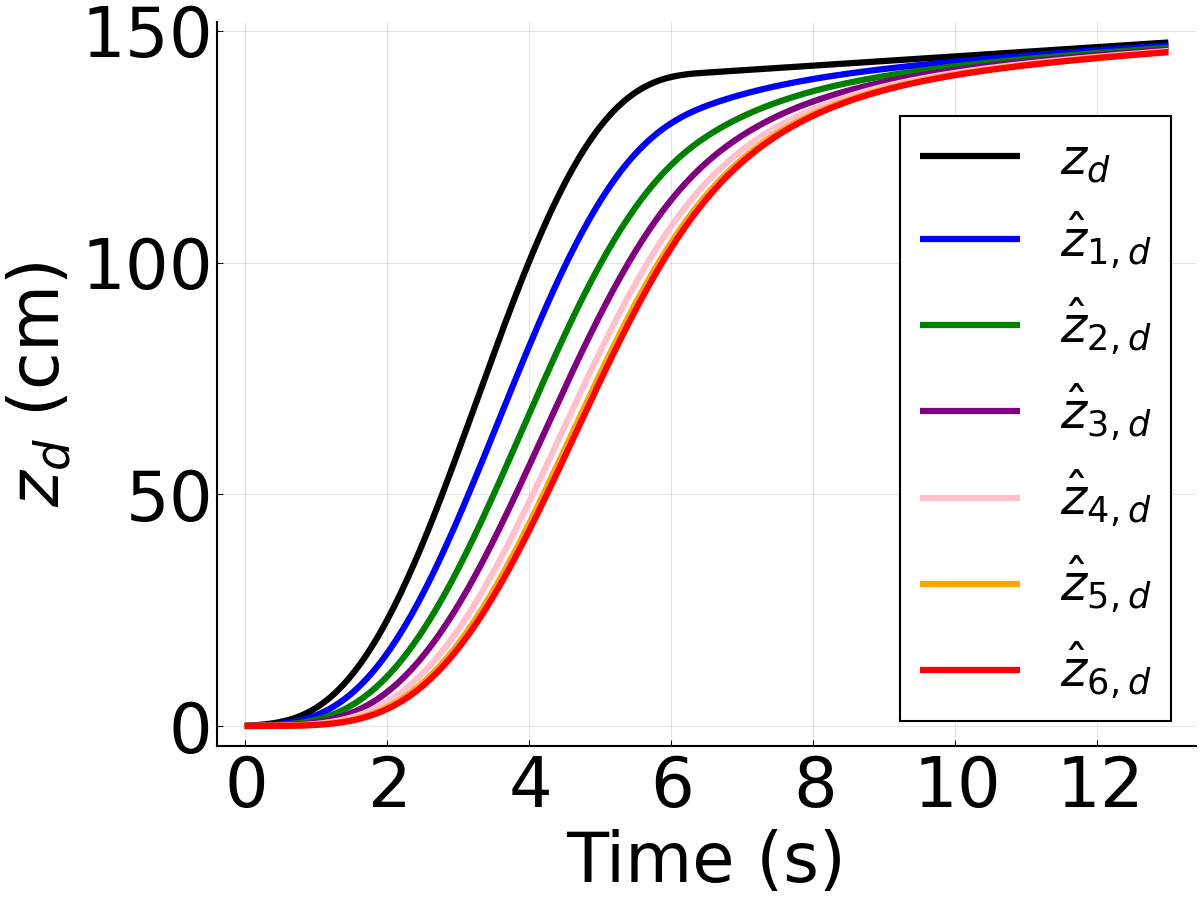
\includegraphics[width=0.42\linewidth]{Figures/standard_quals.png}}
    \hfill
    \subfloat[\label{Fig_dsr}DSR]{%
        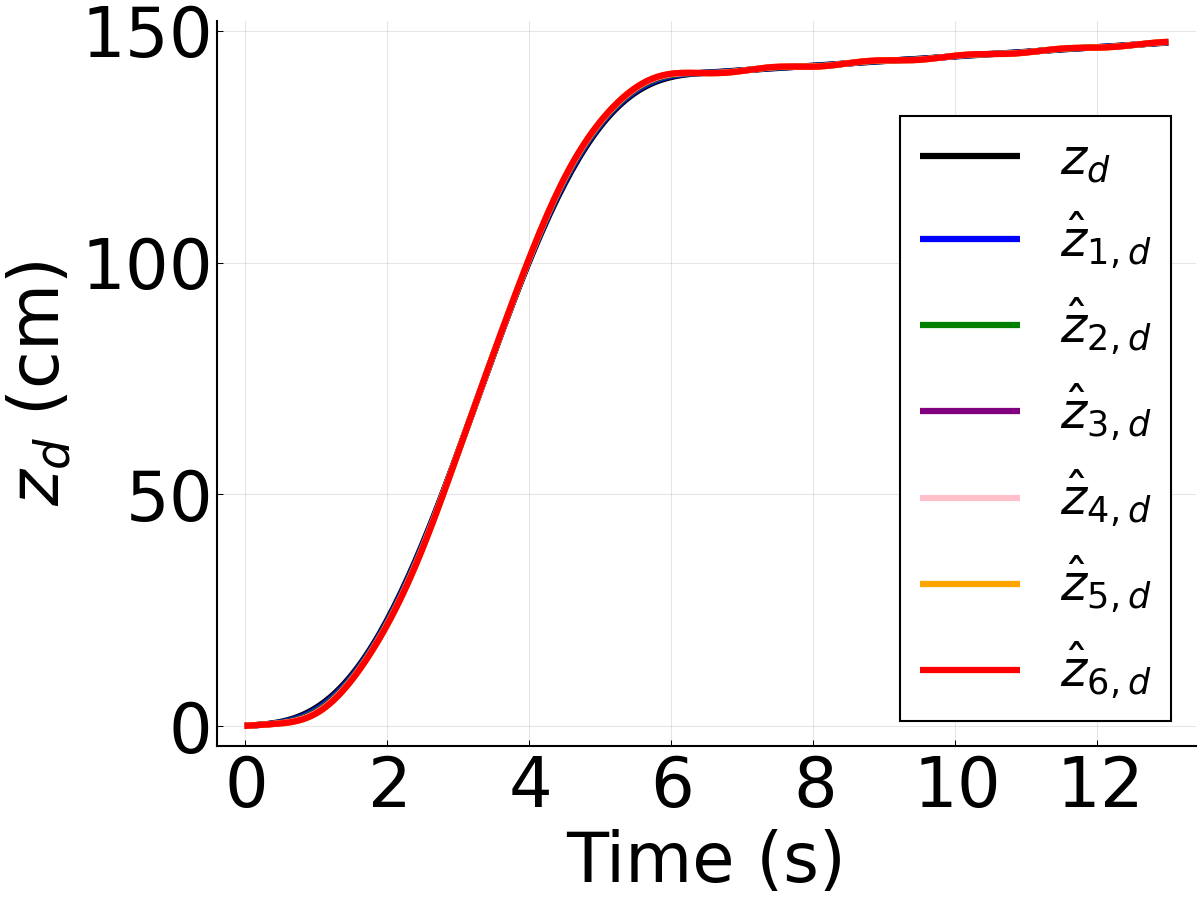
\includegraphics[width=0.42\linewidth]{Figures/dsr_quals.png}}
  \label{Fig_sims} 
\end{figure}
\begin{itemize}
    % \item Potential improvement in decision-making for the dynamic MRTA
    \item Potential improvement for decision-making in time-critical MRTA
\end{itemize}
\end{frame}

\begin{frame}{Research Directions}
    Decentralized decision-making methods for networked systems in dynamic environments
    \begin{columns}
    \begin{column}{0.65\textwidth}
        \begin{enumerate}
        \addtolength{\itemindent}{0.5cm}
        \item Can accurate information communication be maintained in volatile environments?
        \begin{itemize}
            \item Potential approach: Higher-order DSR for communicating information with higher-order dynamics
        \end{itemize}
        \pause
        \item How can learning approaches be utilized to solve dynamic decentralized MRTA problems?
        \begin{itemize}
            \item Current methods treat MRTA problems as static optimization problems and replan each time step.
            \item Potential approach: develop learned policies using multi-agent reinforcement learning by approximating dynamic MRTA problems (lookahead/rollout-based optimization~\cite{bhattacharya2021multiagent}).
            \item Accurate information communication needed for the decentralized policies and modeling   
        \end{itemize}
        \end{enumerate}
        \end{column}
        \begin{column}{0.5\textwidth}
            \includemovie[attach=false,autoplay,text={%
            % 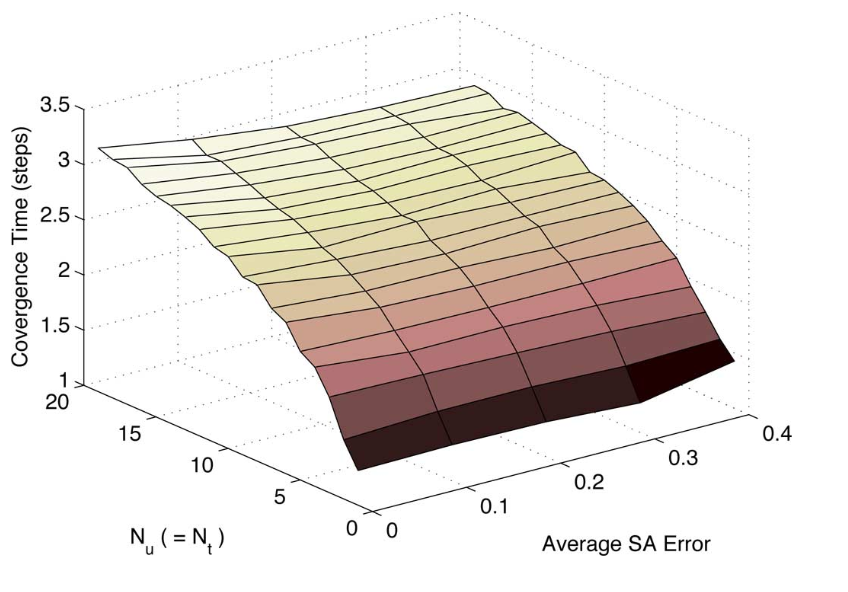
\includegraphics{Figures/convergence_time.png}%
            }]{1.0\linewidth}{1.0\linewidth}{drone_wildfire.gif}
        \end{column}
    \end{columns}
        % \item However, to incorporate dynamics and to account for the rapidly changing environment, I will explore learning methods for policies to general MRTA problems.
        % \item Additionally, I will investigate how DSR can be utilized in the learning process to offer faster learning rates and better policies.
        
        % \item Decentralized networked multi-agent reinforcement learning (MARL) where online policy learning relies on the state of the environment 
\end{frame}

% \begin{frame}
%   \begin{center}
%     \includemovie[attach=false,autoplay,text={%
%         % 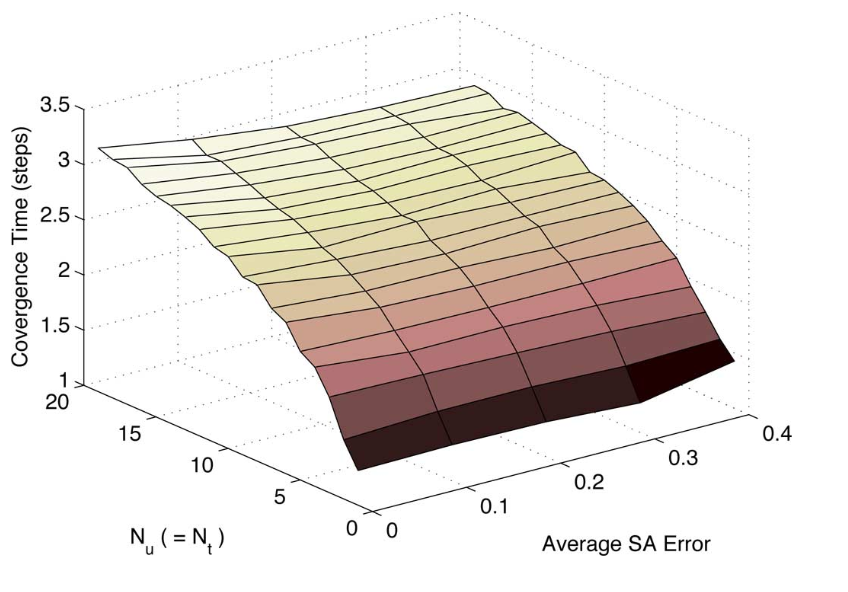
\includegraphics{Figures/convergence_time.png}%
%       }]{1.0\linewidth}{1.0\linewidth}{drone_wildfire.gif}
%   \end{center}
% \end{frame}

\begin{frame}
    \frametitle{Summary}
    \textbf{Presentation content:}
    \begin{itemize}
        \item Literature Review
        \item Paper Review
        \item Research Plan
    \end{itemize}

    \vspace{1cm}
    \textbf{Committee:}
    \begin{itemize}
        \item \textbf{Santosh Devasia} | Faculty Advisor
        \item \textbf{Junlan Wang} | Departmental Representative
        \item \textbf{Xu Chen} | Committee Member
        \item \textbf{Shuonan Dong} | Committee Member
    \end{itemize}

    \vspace{1cm}
    \centering
    \Huge{Questions?}
\end{frame}

\appendix

\begin{frame}[allowframebreaks]{References}
    \bibliographystyle{unsrt}
    \bibliography{ref}
\end{frame}



\end{document}

